\documentclass[letter, 12pt]{article}
\usepackage{comment} % enables the use of multi-line comments (\ifx \fi) 
\usepackage{lipsum} %This package just generates Lorem Ipsum filler text. 
\usepackage{caption}
\usepackage{graphicx}
\usepackage{fullpage} % changes the margin
\usepackage{natbib}
\usepackage{listings}
\lstdefinestyle{blockcode}
{ %Formatting for code in appendix
    language=Java,
    basicstyle=\footnotesize,
    numbers=left,
    stepnumber=1,
    showstringspaces=false,
    tabsize=1,
    breaklines=true,
    breakatwhitespace=false,
}
\lstset
{ %Formatting for code in appendix
    language=Java,
    basicstyle=\footnotesize,
    showstringspaces=false,
    tabsize=1,
    breaklines=true,
    breakatwhitespace=false,
}
\bibliographystyle{abbrvnat}
\setcitestyle{authoryear,open={(},close={)}}
\graphicspath{ {./images/} }

\begin{document}
%Update this information!!!!
\noindent
\large\textbf{CMPT 440 -- Spring 2019: Profanity Filter (Something More?)} \\ \\
\textbf{Christian Santiago} \\
\normalsize   Due Date: 16/5/2019


\section*{Abstract}
The focus of this paper will be on the delta transition creation function that I made. However before this I will briefly discuss the original project idea and implementation. I introduce the complications that come with trying to add increasing amounts of words to the filter manually. I then go into detail regarding my idea for the delta transition creation function and explain how I went about implamenting it. Lastly I will go on about how to further expand its functionalities.

\section*{Introduction}
This project has changed from the original idea of creating a DFA for a maze. My reasoning for changing my project is because I wasn’t to enthusiastic on making a DFA for a maze and it seemed like a pretty linear DFA. As such I decided to work on a Profanity filter instead that could be possibly expanded down the road. I decided to start small and work up from there. The baseline for this idea is to get a statically defined DFA for a set of words I have chosen. I then considered adding to the DFA to make the project a larger undertaking but soon realized the amount of tedious work involved in mapping out at implementing a lager DFA in a transition table. I later discuss how this project changed from just a profanity filter to a general filter generated by a set of words that can be added to a list. The idea change from a simple profanity filter to something more dynamic because I realized that the function that created the DFA only relied on the set of words provided and this meant it was not just restricted to detecting profanity. The reason this expansion was made was because I wanted to have a way to add words in a simple way that did not require me to physically recreate a DFA for each addition I thought of and delta transition table to accommodate for the extra words. I also explain how this function makes the DFA extremely inefficient however I also introduce ideas that may aid in solve this problem. Regardless a DFA using a delta matrix becomes increasingly inefficient for larger and larger alphabets.

\section*{Static DFA Program}
I began creating this dynamic system by starting with a basic case. This base level was a selection of seven words that would be the foundation I would work from. I created the DFA and transition table for the original set of chosen words as seen in Figure \ref{fig:DFA-7w}.
\clearpage
\begin{figure}[!htb]
  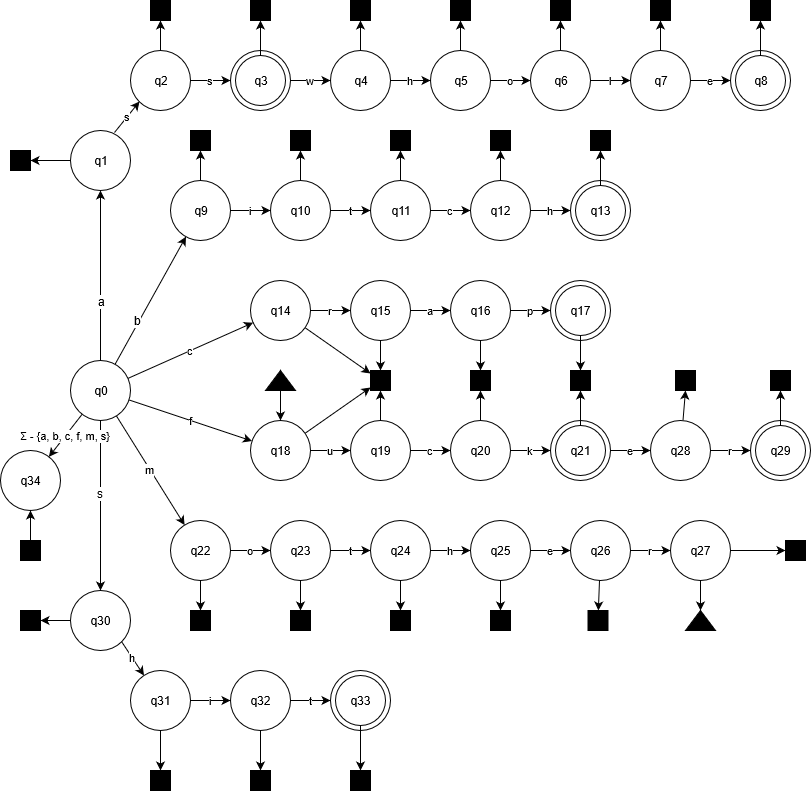
\includegraphics[width=17cm, height=14.5cm, keepaspectratio,]{DFA-Diagram}
  \caption{DFA for 7 words.}
  \label{fig:DFA-7w}
\end{figure} 
This program worked by following the DFA to an accepting state. Looking at the DFA in Figure \ref{fig:DFA-7w}, the starting state is $q_0$ and depending on what input string is given we follow along the transitions until we reach an accepting state or end at a non-accepting state. Our alphabet $\Sigma$ includes all the characters from a-z. The black triangle represents the transition from $q_{27}$ to $q_{18}$ as it contains the same word inside. The black squares represent a transition to the error state $q_{34}$ and having seven words produces a total 35 states. In the original program you would only be able to enter the words that where manually defined beforehand. It can be seen that adding more and more words to this DFA would increase the number of states and complexity of the transition table that is shown in Figure \ref{fig:Table-7w}. At this point adding more words would taking increasing amounts of time and more error prone to incorporate proportional to the words being added.
\begin{figure}[!htb]
  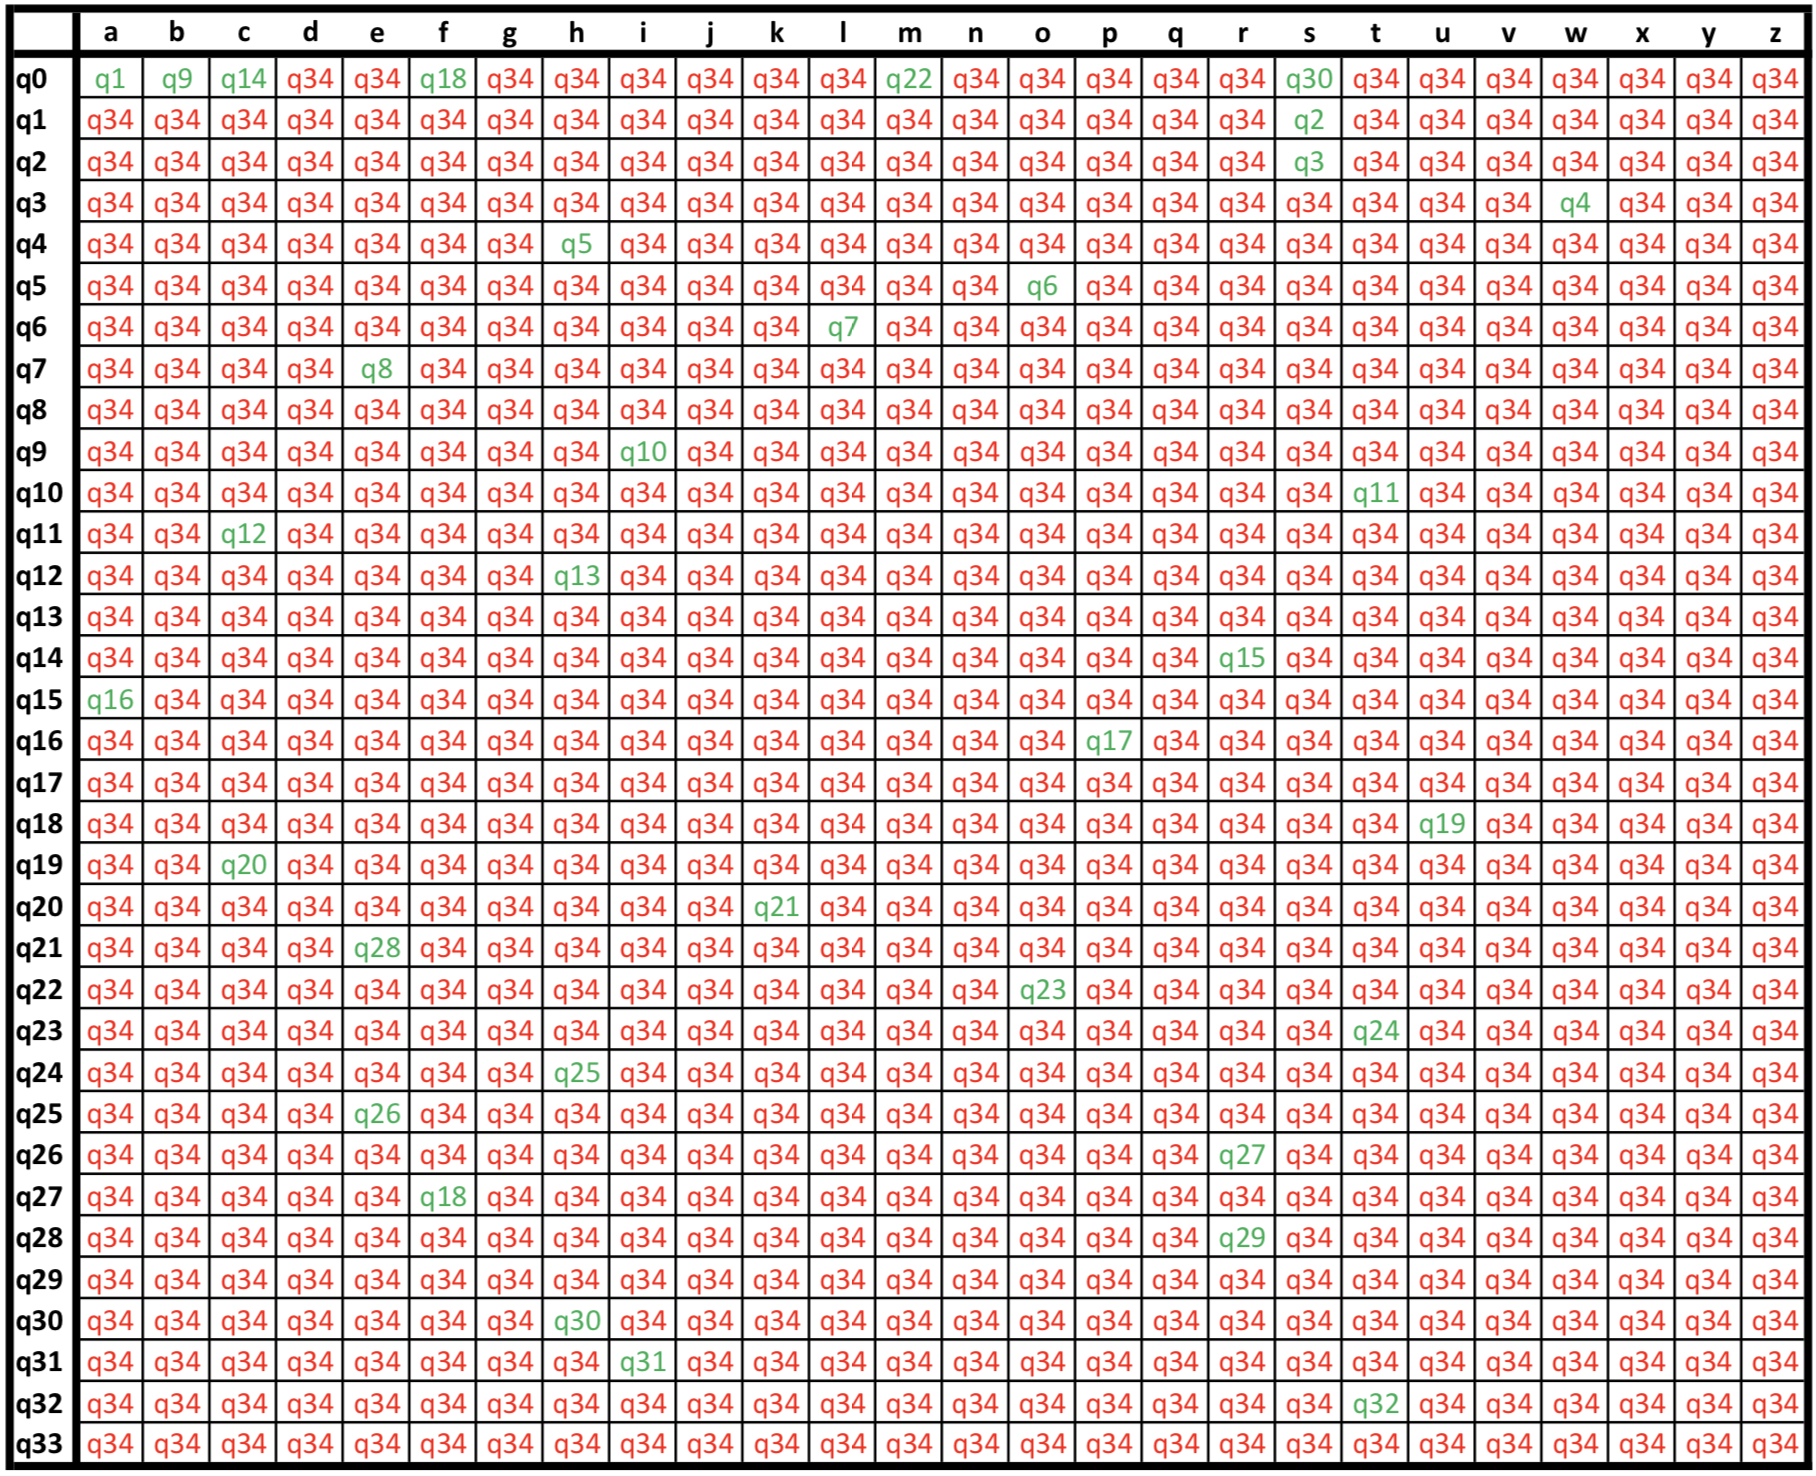
\includegraphics[width=17cm, height=17cm, keepaspectratio,]{table}
  \caption{Transition Table for Figure \ref{fig:DFA-7w}.}
  \label{fig:Table-7w}
\end{figure}
\clearpage

\section*{Dynamic DFA Creation}
The way this was implemented was only possible because of the nature of the ASCII representation and conversion of letters into their decimal counterparts. This idea begins with generalizing the original DFA in Figure \ref{fig:DFA-7w}. We take a conceptual look at what our function would require of us to do dynamically create the delta transition table. Taking a look at Figure 3 we see that from the start state $q_0$ we can go to any state in the set $\{q_1, q_2, q_3, ..., q_{26}\}$ as every word in the english dictionary starts with a letter. Interestingly the index of the states we can go to match the exact position of any letter in the alphabet. Therefore these first 26 states represent the start of any word and we work up from here. As seen in Figure 3 I generalized the possible inputs that we can receive. It turns out that if we use this method to begin our DFA our starting word will always begin and $1 + $ our last created state. At the start this state is $q_{26}$ because this state represents words beginning with $z$. Therefore if we keep track of the state we start at we know the state no matter how long the word is because the end of that word would be at an accepting state and the subsequent state can be used as a starting point for the next new word.This process is just repeated until we have mapped the last word in our list of words.
\begin{figure}[!htb]
  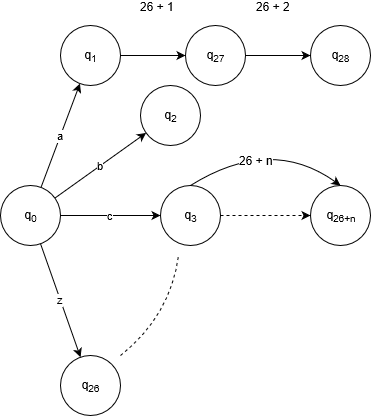
\includegraphics[width=11cm, height=10cm, keepaspectratio,]{AbitraryDFA}
  \caption{DFA with Arbitrary Number of States}
  \label{fig:DFA-A}
\end{figure}

Next I will go in detail in explaining the code and how these ideas were implemented in the function. I begin by introducing the following code.
\begin{lstlisting}[language=Java, caption=Delta Table Creation Function, style=blockcode]

    public void createTransition() {
      int transitions = 0;

      for (String word : wordList) {
        transitions += word.length();
      }
      
      deltaTrans = new int[transitions + 26][26];
      errorState = deltaTrans.length - 1;

      for (int i = 0; i < 26; i ++) {
        deltaTrans[0][i] = i + 1;
      }
      for (int i = 1; i < deltaTrans.length; i ++) {
        for (int j = 0; j < 26; j ++) {
          deltaTrans[i][j] =  errorState;
        }
      }

      transitions = 26;

      for (int d = 0; d < wordList.size(); d ++) {
        for (int i = 0; i < wordList.get(d).length(); i++) {
          char c = wordList.get(d).charAt(i);
          int letter = (int) c;
          int nextState = letter - a;
          try {
            if (i == 0) {
              transState = deltaTrans[0][nextState];
            } else {
                if (deltaTrans[transState][nextState] == errorState) {
                  deltaTrans[transState][nextState] = transitions;
                  if (i + 1 == wordList.get(d).length()) {
                    acceptedStates.add(deltaTrans[transState][nextState]);
                    transitions--;
                  }
                } else {
                  transitions--;
                }
                transState = deltaTrans[transState][nextState];
              }
            } catch (ArrayIndexOutOfBoundsException ex) {
            transState = errorState;
          }
          transitions++;
        }
      }
    }
\end{lstlisting}
We begin by initializing our matrix. We reset our number of transitions to 0 since our DFA is not created yet.
\begin{lstlisting}[language=Java]
      int transitions = 0;
\end{lstlisting}
We then calculate the number of transitions that are going to take place. This can also be understood as the number of states there are. 
 \begin{lstlisting}[language=Java]
      for (String word : wordList) {
        transitions += word.length();
      }
\end{lstlisting}
Since we already know that we are reserving the states $q_1$ to $q_26$ for the letters of the alphabet we create states equal to 26 plus the transitions we calculated and our alphabet is limited to letters so there are only 26 positions for each array. Following this we assign our error state as the last state in the matrix. 
\begin{lstlisting}[language=Java]
      deltaTrans = new int[transitions + 26][26];
      errorState = deltaTrans.length - 1;
\end{lstlisting} 
We set up our transitions for the starting state 
\begin{lstlisting}[language=Java]
      for (int i = 0; i < 26; i ++) {
        deltaTrans[0][i] = i + 1;
      }
\end{lstlisting}
and we go through the rest of the states and fill the transitions with error states.
\begin{lstlisting}[language=Java]
      for (int i = 1; i < deltaTrans.length; i ++) {
        for (int j = 0; j < 26; j ++) {
          deltaTrans[i][j] =  errorState;
        }
      }
\end{lstlisting}

Now that our matrix is setup we begin with the modification process. We start by reseting our transition marker to $q_{26}$ as this is the last known state in position $z$. 
\begin{lstlisting}[language=Java]
      transitions = 26;
\end{lstlisting}
The purpose of the outer most for loop on is to go through the list of words until we reach the last word. 
\begin{lstlisting}[language=Java]
      for (int d = 0; d < wordList.size(); d ++) {
\end{lstlisting}
The inner for loop lets us process the word we are currently on character by character until we reach the end of the word and increment transitions to signify a new state will be created and set to this state.
\begin{lstlisting}[language=Java]
        for (int i = 0; i < wordList.get(d).length(); i++) {
        ...
        transitions++
        }
\end{lstlisting}
Then we take advantage of the fact that the alphabet is limited to letters and use that to calculate where is our next goto position would be within the state.
\begin{lstlisting}[language=Java]
          char c = wordList.get(d).charAt(i);
          int letter = (int) c;
          int nextState = letter - a;
\end{lstlisting}
 We then use a try catch statement to prevent any out of bounds errors and just assign the current state to the error state.
 \begin{lstlisting}[language=Java]
          try {
            ...
          } catch (ArrayIndexOutOfBoundsException ex) {
            transState = errorState;
          }
\end{lstlisting}
Next check if we are currently in the first letter of the word. In this case we already created a state that represents this transition. So we assign our transition state to the appropriate state for any given letter.
\begin{lstlisting}[language=Java]
            if (i == 0) {
              transState = deltaTrans[0][nextState];
            }
\end{lstlisting}
Otherwise we begin to calculate our transition path. This begins by checking if the state we try to go to is an error state. If it is an error state this means no path has been created yet so we will make one by changing this error state to the next state. If we have already mapped a path to the next state then follow that path instead of creating a duplicate path. This is was the transitions-- signifies.
\begin{lstlisting}[language=Java]
            } else {
                if (deltaTrans[transState][nextState] == errorState) {
                  deltaTrans[transState][nextState] = transitions;
                  ...
                } else {
                    transitions--;
                  }
\end{lstlisting}
However we must also keep track of our accepting state. We do so by checking if the letter we are on is at the end of the word. If it is this means we should mark this state as an accepting state. Also decrement transitions to correct the transitions count as the current state will be used as an accepting state.
\begin{lstlisting}[language=Java]
                  if (i + 1 == wordList.get(d).length()) {
                    acceptedStates.add(deltaTrans[transState][nextState]);
                    transitions--;
                  }
\end{lstlisting}
Finally set our current state to the next state to restart the calculation process for the next state.
\begin{lstlisting}[language=Java]
                transState = deltaTrans[transState][nextState];
\end{lstlisting}

I will end with an example of how this works. Let us take a random word to add to our list. Let us assume this word is "buy." Since our word list consist of only the work "buy" we go through the outer loop once and because our word is 3 letter long we iterate through the inner loop 3 times. Our first character is 'b' and 'b' - 'a' = 1. Since we are on the first letter we get the following deltaTrans[0][1] = 2 which is assigned to our transState or current state and transitions is incremented to 27. We now have the letter 'u' and calculate 'u' - 'a' = 20. We are not on the first letter and currently deltaTrans[2][20] is at our error state since we have not processed any other words so we know it is at the initial error state. Therefore we remap this previously $deltaTrans[2][20] = error state$ to $deltaTrans[2][20] = transitions$ which is currently 27 and then increment transitions to 28. Finally we reassign transState to the new deltaTrans[2][20] which is 27. We now reach the letter 'y' and calculate 'y' - 'a' = 24. We check if deltaTrans[27][24] is an error state. It is because everything was initialized to the error state. deltaTrans[27][24] = transitions which is remapped to 28 now.  We are at the end of the word so we add deltaTrans[27][24] which was remapped to 28, 28 becomes an accepting state and we decrement transitions to 27. In the end transState = deltaTrans[27][24] which is 28 and transitions gets incremented to 28. We have ended the creation of our delta matrix and the word "buy" is now an accepted word by our program. As you can see we started at 26 but did not map anything to this state because we skip mapping for the first letter and therefore 28 is not in danger of being incorrectly remapped either.

\section*{User Manual}
To use this system you begin by opening the command line and and change your directory to the directory if the java class file. Then run the program by entering 
\lstinline{java driverDFA}
The current word list will be presented and you will then be prompted to enter any new words you would like to add to the list. After you type \lstinline{exit} to leave input word list mode you will then be in the check words mode. The new word list will be presented and you may now try to enter words allowed or not allowed and it will tell you if it is or isn't. You can exit at any time my typing \lstinline{exit}.
 
\section*{Conclusion}
I have shown how a DFA  transition table can be created from a list of words that can be added or removed. This process was only possible because of the nature of the letters and their ASCII decimal conversions. If not for this there would have to be extra work involved in determining what position any letter can be in. However this function does have its limitations. By nature of a delta matrix transition increasingly larger alphabets and words use more memory. There could be a lot of wasted memory as well if words have other words contained in them and therefore waist space in the assignment of memory when initializing the delta transition table. With slight modifications some of its issues can be resolved and even improved. In conclusion this is a fantastic project that can dynamically create the delta transition table for any list of words so any sort of filter that one wanted as long as it only pertained to letters at the moment can be created by this function. 

% This is how you cite
%	\cite{Gudder2000}
%	\cite{Brodsky}



%=============================================
\bibliographystyle{acl}
\bibliography{Cites.bib}

\end{document}


\ifx
Comments!
\fi

% ===========

\ifx

%==============

% References if you want it manual

% \bibitem{Robotics} Fred G. Martin \emph{Robotics Explorations: A Hands-On Introduction to Engineering}. New Jersey: Prentice Hall.

% \bibitem{Flueck}  Flueck, Alexander J. 2005. \emph{ECE 100}[online]. Chicago: Illinois Institute of Technology, Electrical and Computer Engineering Department, 2005 [cited 30
% August 2005]. Available from World Wide Web: (http://www.ece.iit.edu/~flueck/ece100).

